\section{Hierarchical Basis and Hierarchical Subspace}
\label{sec:22hierSubspaces}

\minitoc{67mm}{5}

\noindent
The dimension of the nodal space $\ns{\*l}$ is given by
\begin{equation}
  \label{eq:dimensionFG}
  \dim \ns{\*l}
  = \setsize{\fgset{\*l}}
  = \prod_{t=1}^d (2^{l_t} + 1).
\end{equation}
If we choose the same level $n \in \natz$ in all dimensions,
then the dimension of $\ns{n,d}$ and the
number of grid points grow at least as fast as
$2^{nd} = (\ms{n}^{-1})^d$.
This exponential dependency between $\dim \ns{n,d}$ and $d$ is known as the
\term{curse of dimensionality} \cite{Bellman61Adaptive}.
The curse makes interpolation on $\ns{\*l}$ computationally infeasible
for dimensionalities $d > 4$,
as we would have to calculate and store
$\dim(\ns{\*l})$-many coefficients $\interpcoeff{\*l,\*i}$.%



\subsection{Hierarchical Splitting in the Univariate Case}
\label{sec:221hierUV}

\paragraph{Hierarchical subspaces}

In order to reduce the computational effort,
we first split $\ns{\*l}$ into smaller subspaces and then identify
subspaces that we can omit at the cost of a slightly larger error.
In the univariate case, the key observation is that a grid point of a
level $l$ can be written as a grid point of a higher level~$l'$:
\begin{equation}
  \label{eq:rewriteGridPoint}
  \gp{l,i} = \gp{l',i'},\quad
  l' \ge l,\quad
  i' = 2^{l'-l} i.
\end{equation}
Conversely, this implies that every grid point $\gp{l,i}$ of level $l \ge 1$
and index $i \ge 1$ can be uniquely written
as a grid point of a coarser level $l'$ (or $l' = l$) and an odd index $i'$:
\begin{equation}
  \gp{l,i} = \gp{l',i'},\quad
  l' = l - \bracket*{\log_2(\xor(i, i-1) + 1) - 1},\quad
  i' = 2^{l'-l} i,
\end{equation}
where $\xor$ is the bitwise ``exclusive or'' function.
The term in square brackets is the exponent of the
highest power of two that divides $i$.
The two boundary points zero and one are obtained by
inserting an additional level $l' = 0$ with indices $i' \in \{0, 1\}$.
As shown in \cref{fig:pointSplittingUniform},
this implies that $\fgset{l}$ decomposes into
\begin{equation}
  \fgset{l}
  = \bigdotcup_{l'=0}^l \{\gp{l',i'} \mid i' \in \hiset{l'}\},\quad
  \hiset{l'} \ceq
  \begin{cases}
    \{i' = 0, \dotsc, 2^{l'} \mid \text{$i'$ odd}\},&l' > 0,\\
    \{0, 1\},&l' = 0,
  \end{cases}
\end{equation}
where $\dotcup$ indicates the disjoint union.
We call the spaces spanned by the basis functions that correspond to the
index sets $\hiset{l'}$ \term{hierarchical subspaces} $\hs{l'}$:
\begin{equation}
  \hs{l'}
  \ceq \spn\{\basis{l',i'} \mid i' \in \hiset{l'}\}.
\end{equation}
The corresponding basis functions
$\basis{l',i'}$, $l' = 0, \dotsc, l$, $i' \in \hiset{l'}$,
are called \term{hierarchical basis functions.}
The hierarchical hat function basis is shown in \cref{fig:hierarchicalHat}.

\begin{SCfigure}
  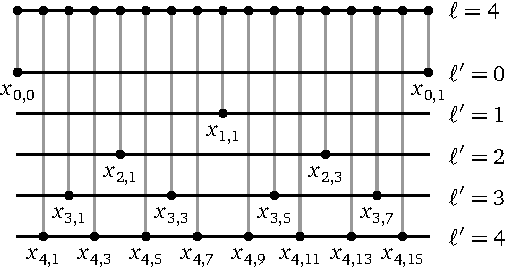
\includegraphics{pointSplitting_1}%
  \caption[%
    Decomposition of the set of univariate grid points%
  ]{%
    The set of grid points $\fgset{l}$ of level $l = 4$ \emph{(top)}
    decomposes into hierarchical grids of level $l' \le l$,
    whose grid points $\gp{l',i'}$ have odd indices $i' \in \hiset{l'}$
    ($\gp{0,0}$ being the only exception).%
  }%
  \label{fig:pointSplittingUniform}%
\end{SCfigure}

\begin{figure}
  \subcaptionbox{%
    Basis functions $\bspl{l',i'}{1}$ ($l' \le l$, $i' \in \hiset{l'}$)
    and grid points $\gp{l',i'}$ \emph{(dots).}
    The domain is the unit interval $\clint{0, 1}$.%
  }[72mm]{%
    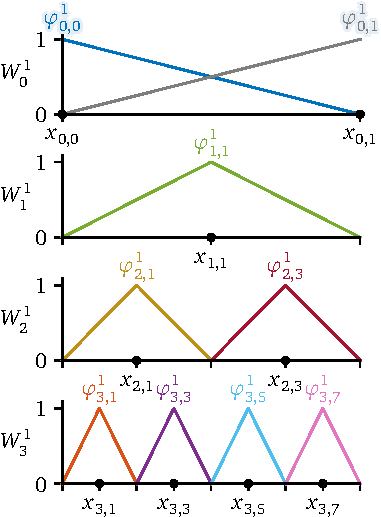
\includegraphics{hierarchicalBasis_2}%
  }%
  \hfill%
  \subcaptionbox{%
    Piecewise linear interpolant $\fgintp{l}$
    of some function data $\objfun(\gp{\*l,\*i})$
    as a linear combination of hierarchical hat functions \emph{(stacked).}
    The two boundary functions are combined to a single function
    \emph{\textcolor{C0}{(blue)}} for simplicity.%
  }[72mm]{%
    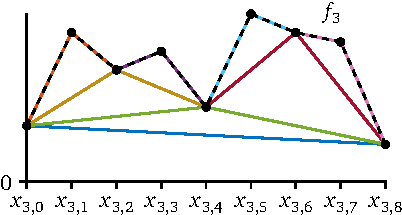
\includegraphics{interpolant_2}%
  }%
  \caption[%
    Univariate hierarchical hat functions%
  ]{%
    Univariate hierarchical hat functions up to level $l = 3$.%
  }%
  \label{fig:hierarchicalHat}%
\end{figure}

\paragraph{Hierarchical splitting}

For the hat function basis $\bspl{l,i}{1}$ and other basis types,
we can prove that the corresponding nodal space
decomposes into the direct sum of all
hierarchical subspaces of coarser levels or the same level, i.e.,
\begin{equation}
  \label{eq:hierSplittingUV}
  \ns{l}
  \overset{?}{=} \bigoplus_{l'=0}^l \hs{l'}.
\end{equation}
We call this relation \term{hierarchical splitting.}
Here, the direct sum $\oplus$ is
the vector space sum that additionally indicates
that the dimension of the sum $\sum_{l'=0}^l \hs{l'}$ is the sum
of the dimensions of the summands $\hs{l'}$
(analogously to
$\setsize{\fgset{l}}
= \sum_{l'=0}^l \setsize{\{\gp{l',i'} \mid i' \in \hiset{l'}\}}$,
where $\fgset{l}$ is the disjoint union of the sets
$\{\gp{l',i'} \mid i' \in \hiset{l'}\}$).
In general, \eqref{eq:hierSplittingUV} may not be true,
depending on the type of basis functions.
The following lemma provides a characterization
that can be used to prove \eqref{eq:hierSplittingUV} for hat functions.

\vspace*{\fill}
\pagebreak

\begin{lemma}[univariate hierarchical splitting characterization]
  \label{lemma:hierSplittingUV}
  \Cref{eq:hierSplittingUV} is equivalent to the satisfaction of
  both of the following conditions:
  \begin{itemize}
    \item
    The hierarchical subspaces $\hs{l'}$ ($l' \le l$)
    are subspaces of $\ns{l}$.
    
    \item
    The hierarchical functions
    $\basis{l',i'}$ ($l' \le l$, $i' \in \hiset{l'}$)
    are linearly independent.
  \end{itemize}
\end{lemma}
\begin{proof}
  The first condition is equivalent to $\sum_{l'=0}^l \hs{l'} \subset \ns{l}$.
  The second condition is equivalent to
  $\dim \sum_{l'=0}^l \hs{l'} = \sum_{l'=0}^l \dim \hs{l'}$,
  i.e., to the directness of the sum.
  Therefore, the logical conjunction of both is equivalent to
  $\bigoplus_{l'=0}^l \hs{l'} \subset \ns{l}$.
  If the sum is direct,
  the dimension of the sum is equal to $2 + \sum_{l'=1}^l 2^{l'-1} = 2^l + 1$
  (due to $\dim \hs{l'} = \setsize{\hiset{l'}} = 2^{l'-1}$ for $l' > 0$ and
  $\dim \hs{l'} = 2$ for $l' = 0$),
  which is also the dimension of $\ns{l}$.
  The only subspace of $\ns{l}$ that has the same
  dimension as $\ns{l}$ is $\ns{l}$ itself,
  so we infer $\bigoplus_{l'=0}^l \hs{l'} = \ns{l}$.
\end{proof}
\begin{corollary}[univariate hierarchical splitting for hat functions]
  \label{cor:hierSplittingHatUV}
  The hierarchical splitting \eqref{eq:hierSplittingUV}
  holds for the hat function basis.
\end{corollary}
\begin{proof}
  The first condition of \cref{lemma:hierSplittingUV}
  is satisfied as piecewise linear splines of level~$l'$
  are also piecewise linear splines of higher levels $l \ge l'$.
  We can prove the linear independence for the second condition by induction
  over $l$:
  If a linear combination of $\bspl{l',i'}{1}$
  ($l' \le l$, $i' \in \hiset{l'}$)
  vanishes everywhere, then the coefficients of level $l$ must be zero,
  as otherwise the basis functions $\bspl{l,i'}{1}$ ($i' \in \hiset{l}$) would
  introduce kinks at $\gp{l,i'}$, which the zero function does not have.
  This means that we have a zero linear combination of $\bspl{l',i'}{1}$ for
  $l' \le l - 1$, $i' \in \hiset{l'}$,
  and by the induction hypothesis, the other coefficients also vanish.
\end{proof}



\subsection{Hierarchical Splitting in the Multivariate Case}
\label{sec:222hierMV}

Multivariate hierarchical subspaces are defined analogously
to the univariate case:
\begin{equation}
  \hs{\*l}
  \ceq \spn\{\basis{\*l,\*i} \mid \*i \in \hiset{\*l}\},\quad
  \hiset{\*l}
  \ceq \hiset{l_1} \times \dotsb \times \hiset{l_d},\quad
  \*l \in \natz^d.
\end{equation}
The univariate hierarchical splitting \eqref{eq:hierSplittingUV}
can now be generalized to
\begin{equation}
  \label{eq:hierSplittingMV}
  \ns{\*l}
  \overset{?}{=} \bigoplus_{\*l'=\*0}^\*l \hs{\*l'}.
\end{equation}
Again, this relation does not hold in general.
We use a multivariate counterpart of \thmref{lemma:hierSplittingUV}
to prove that \eqref{eq:hierSplittingMV} holds if
the corresponding univariate relation \eqref{eq:hierSplittingUV}
holds for all dimensions:

\begin{lemma}[multivariate hierarchical splitting characterization]
  \label{lemma:hierSplittingMV}
  \Cref{eq:hierSplittingMV} is equivalent to the satisfaction of
  both of the following conditions:
  \begin{itemize}
    \item
    The hierarchical subspaces $\hs{\*l'}$ ($\*l' \le \*l$)
    are subspaces of $\ns{\*l}$.
    
    \item
    The basis functions
    $\basis{\*l',\*i'}$ ($\*l' \le \*l$, $\*i' \in \hiset{\*l'}$)
    are linearly independent.
  \end{itemize}
\end{lemma}

\vspace*{0pt plus 0.3fill}

\begin{proof}
  If the sum is direct, then its dimension is given by
  \begin{equation}
    \hspace*{-5mm}
    \dim \sum_{\*l'=\*0}^\*l \hs{\*l'}
    = \sum_{l_1'=0}^{l_1} \dotsb \sum_{l_d'=0}^{l_d}
    \prod_{t=1}^d \dim \hs{l_t'}
    = \prod_{t=1}^d \sum_{l_t'=0}^{l_t} \dim \hs{l_t'}
    = \prod_{t=1}^d (2^{l_t} + 1)
    = \dim \ns{\*l}
    \hspace*{-5mm}
  \end{equation}
  using \eqref{eq:dimensionFG}.
  The rest is analogous to the proof of \cref{lemma:hierSplittingUV}.
\end{proof}

\vspace*{0pt plus 1fill}

\begin{proposition}[from univariate to multivariate splitting]
  \label{prop:splittingUVToMV}
  If univariate splitting \eqref{eq:hierSplittingUV}
  holds for every dimension,
  then the multivariate splitting \eqref{eq:hierSplittingMV} holds as well.
\end{proposition}

\vspace*{0pt plus 0.3fill}

\begin{proof}
  We check the two conditions of \cref{lemma:hierSplittingMV}
  given the two univariate conditions of \cref{lemma:hierSplittingUV}:
  \begin{enumerate}
    \item
    The hierarchical basis functions $\basis{\*l',\*i'}$
    of $\hs{\*l'}$ ($\*l' \le \*l$, $\*i' \in \hiset{\*l'}$)
    are tensor products of functions $\basis{l_t',i_t'}$.
    According to the first condition of \cref{lemma:hierSplittingUV},
    each $\basis{l_t',i_t'}$ can be written as a linear combination of
    the nodal basis $\basis{l_t,i_t}$ ($i_t = 0, \dotsc, 2^{l_t}$).
    We can expand the tensor product to a linear combination
    of tensor products of the univariate nodal basis functions.
    Therefore, $\basis{\*l',\*i'}$ is a linear combination of
    multivariate nodal functions, i.e., $\basis{\*l',\*i'} \in \ns{\*l}$.
    As this is true for all $\*i' \in \hiset{\*l'}$, we obtain
    $\hs{\*l'} \subset \ns{\*l}$.
    
    \item
    The linear independence of the hierarchical functions $\basis{\*l',\*i'}$
    ($\*l' \le \*l$, $\*i' \in \hiset{\*l'}$) can be shown completely
    analogously to the proof of
    \thmref{lemma:tensorProductLinearIndependence}.
  \end{enumerate}
  According to \cref{lemma:hierSplittingMV},
  the multivariate splitting \eqref{eq:hierSplittingMV} holds.
\end{proof}

\vspace*{0pt plus 1fill}

A direct consequence of \cref{prop:splittingUVToMV} is that
the hierarchical splitting holds for the hierarchical hat function basis.

\pagebreak

\begin{corollary}[multivariate hierarchical splitting for hat functions]
  \label{cor:hierSplittingHatMV}
  The multivariate hierarchical splitting \eqref{eq:hierSplittingMV}
  holds for the hat function basis.
\end{corollary}
\begin{proof}
  Follows directly by applying
  \thmref{cor:hierSplittingHatUV} to \cref{prop:splittingUVToMV}.
\end{proof}
